% 5.3：依据表1、表2与同源的已保存数值场分析结果；图3、图4均使用用户提供的PNG。
\subsection{结果分析}
\label{sec:p1-analysis}

\subsubsection{温度分布与升温滞后}

图\ref{fig:p1-temperature}显示，高温区域由表面向内部扩展，中心升温滞后。
$1800\ \mathrm{s}$时，中心与表面温度分别为$33.5753\tempunit$、$36.7856\tempunit$，
径向温差为$3.2103\tempunit$，表面仍比环境低约$4.73\tempunit$。

\begin{figure}[!htbp]
\centering
% 保持原图3的0.98\textwidth宽度及264.543625/636.93875高宽比。
% 裁去白边并压缩(a)主图与色条的间距，扩展主图裁剪以保留横排刻度及纵轴文字。
% trim按源PNG的300 dpi换算；各部分仅指定高度，保持原始比例和图组占位。
\setlength{\unitlength}{0.98\textwidth}
\begin{picture}(1,0.41533605)
  % A
  \put(0.015715190,0.004523636){\makebox(0,0)[lb]{%
    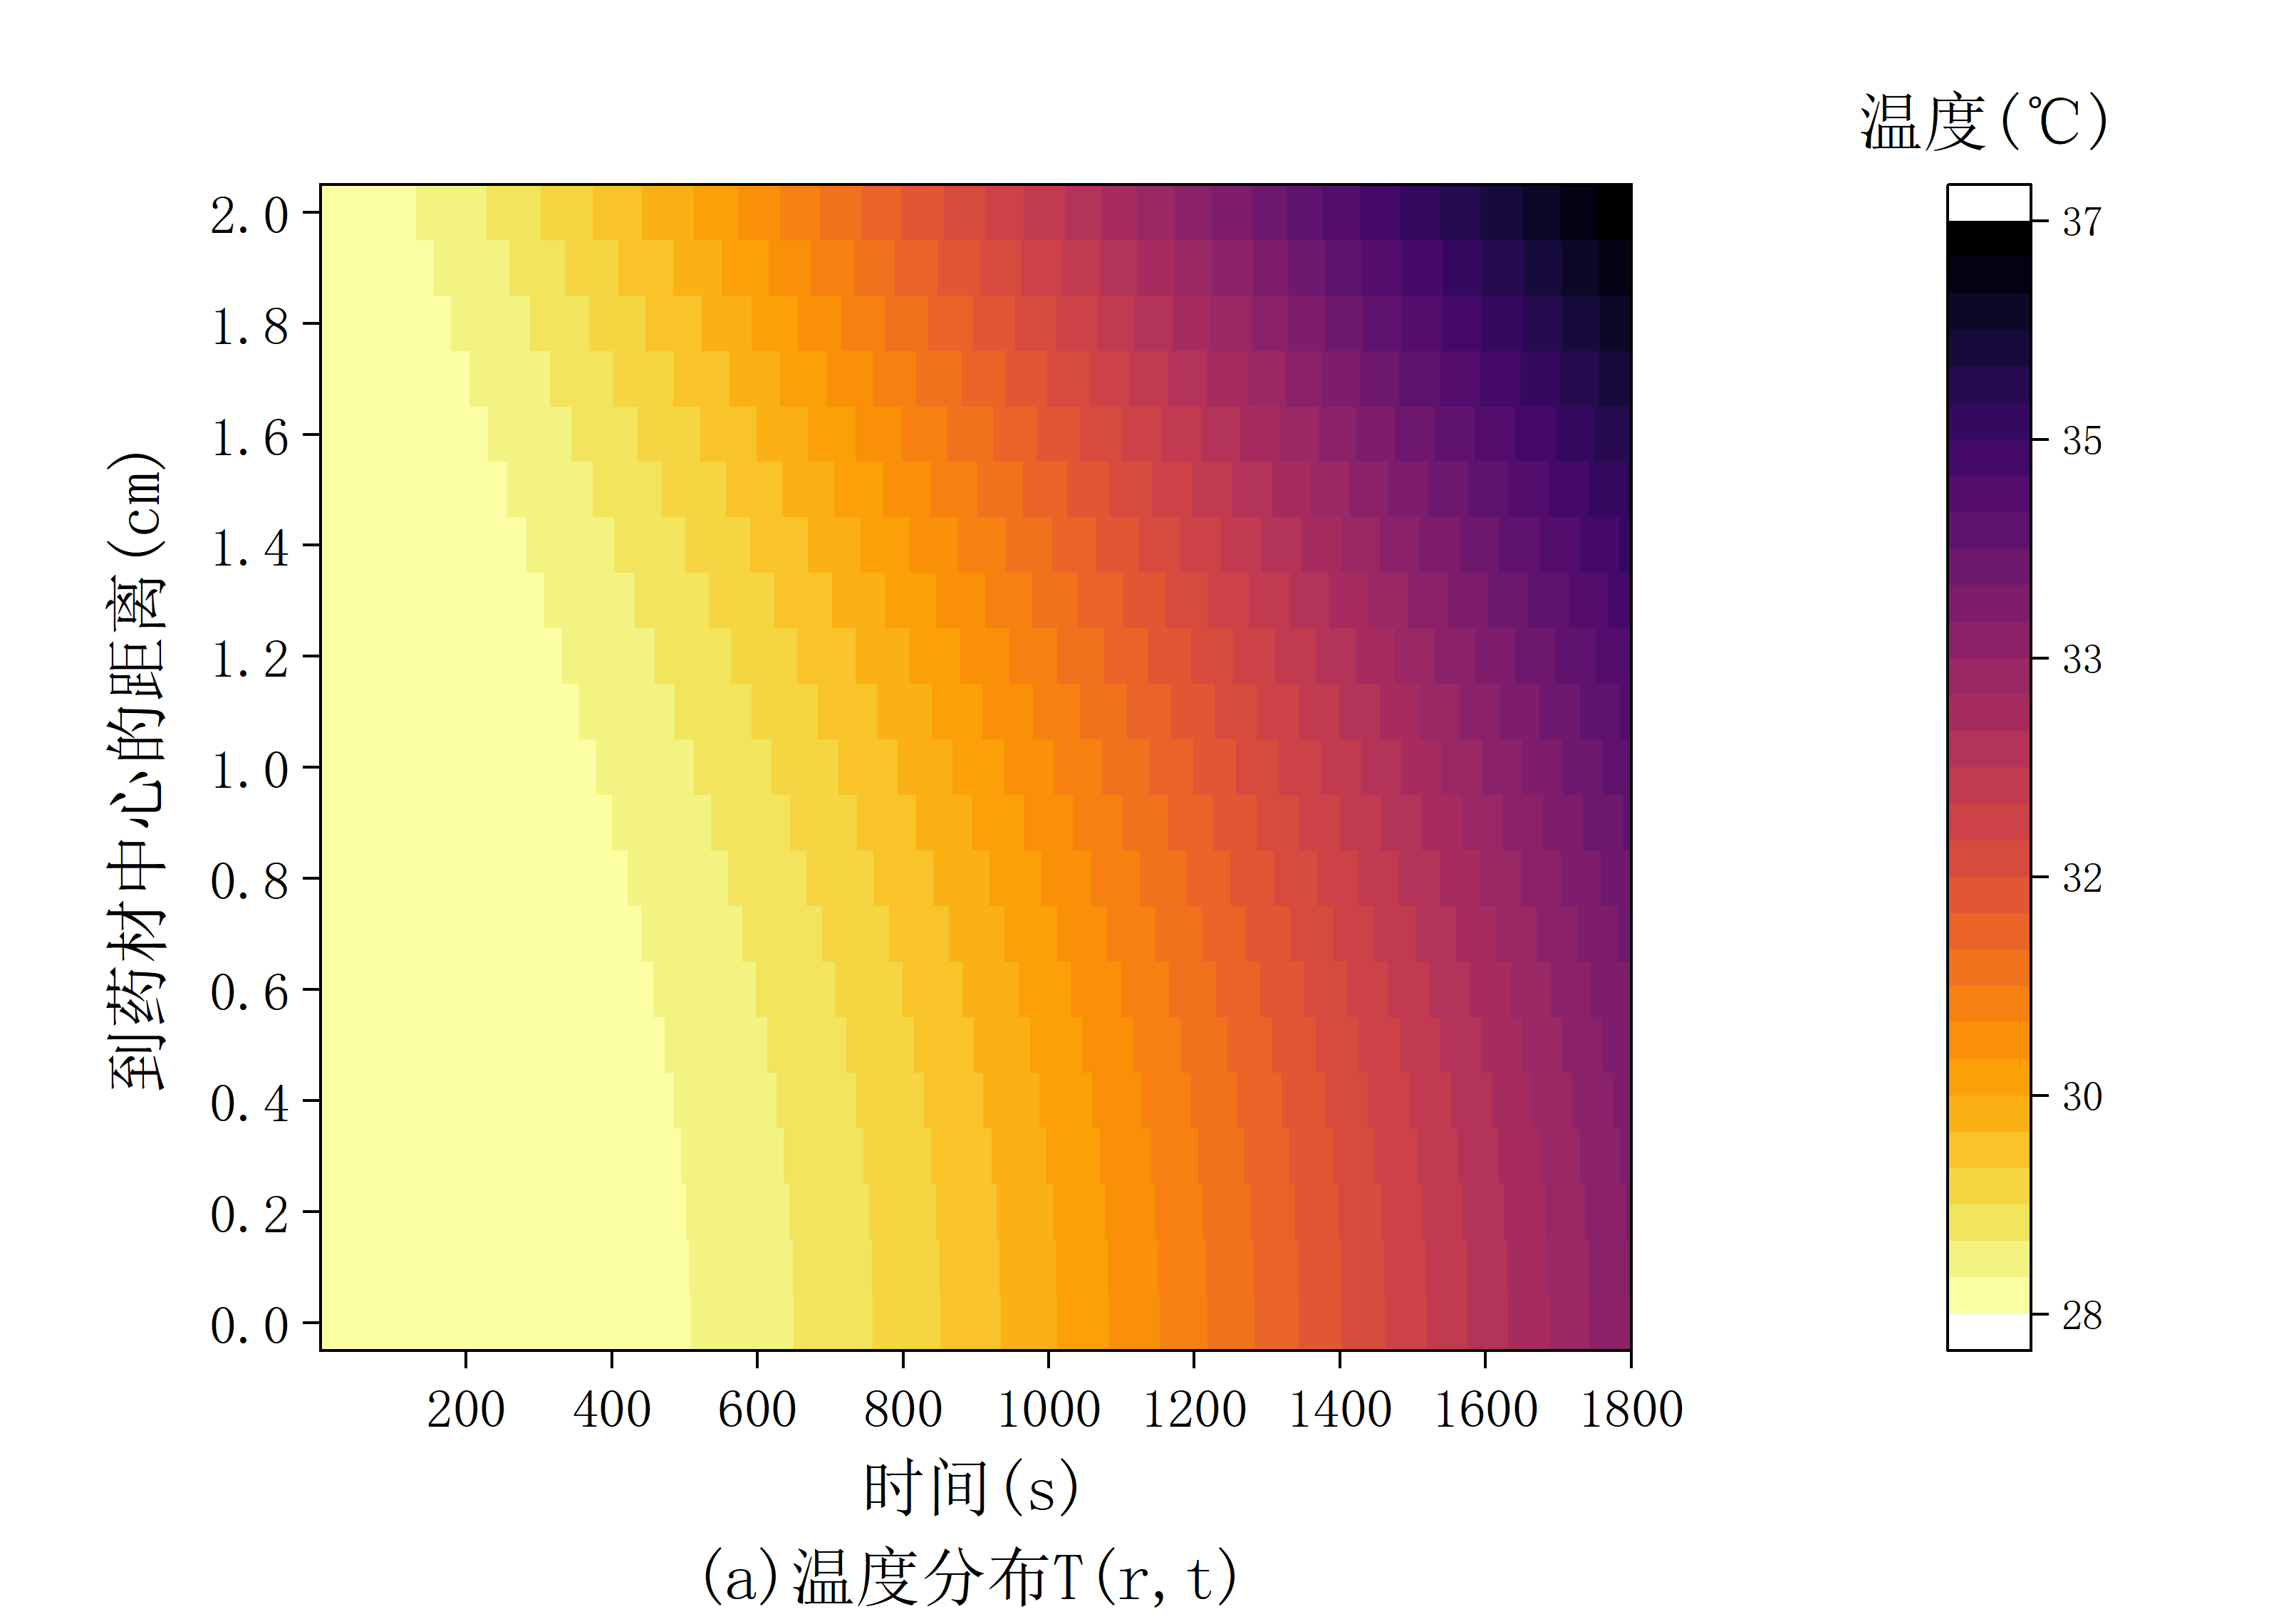
\includegraphics[trim={32.400bp 26.400bp 200.640bp 32.400bp},clip,
      height=0.400352928\unitlength]{图4(a).png}}}
  % Colorbar
  \put(0.443173632,0.053707042){\makebox(0,0)[lb]{%
    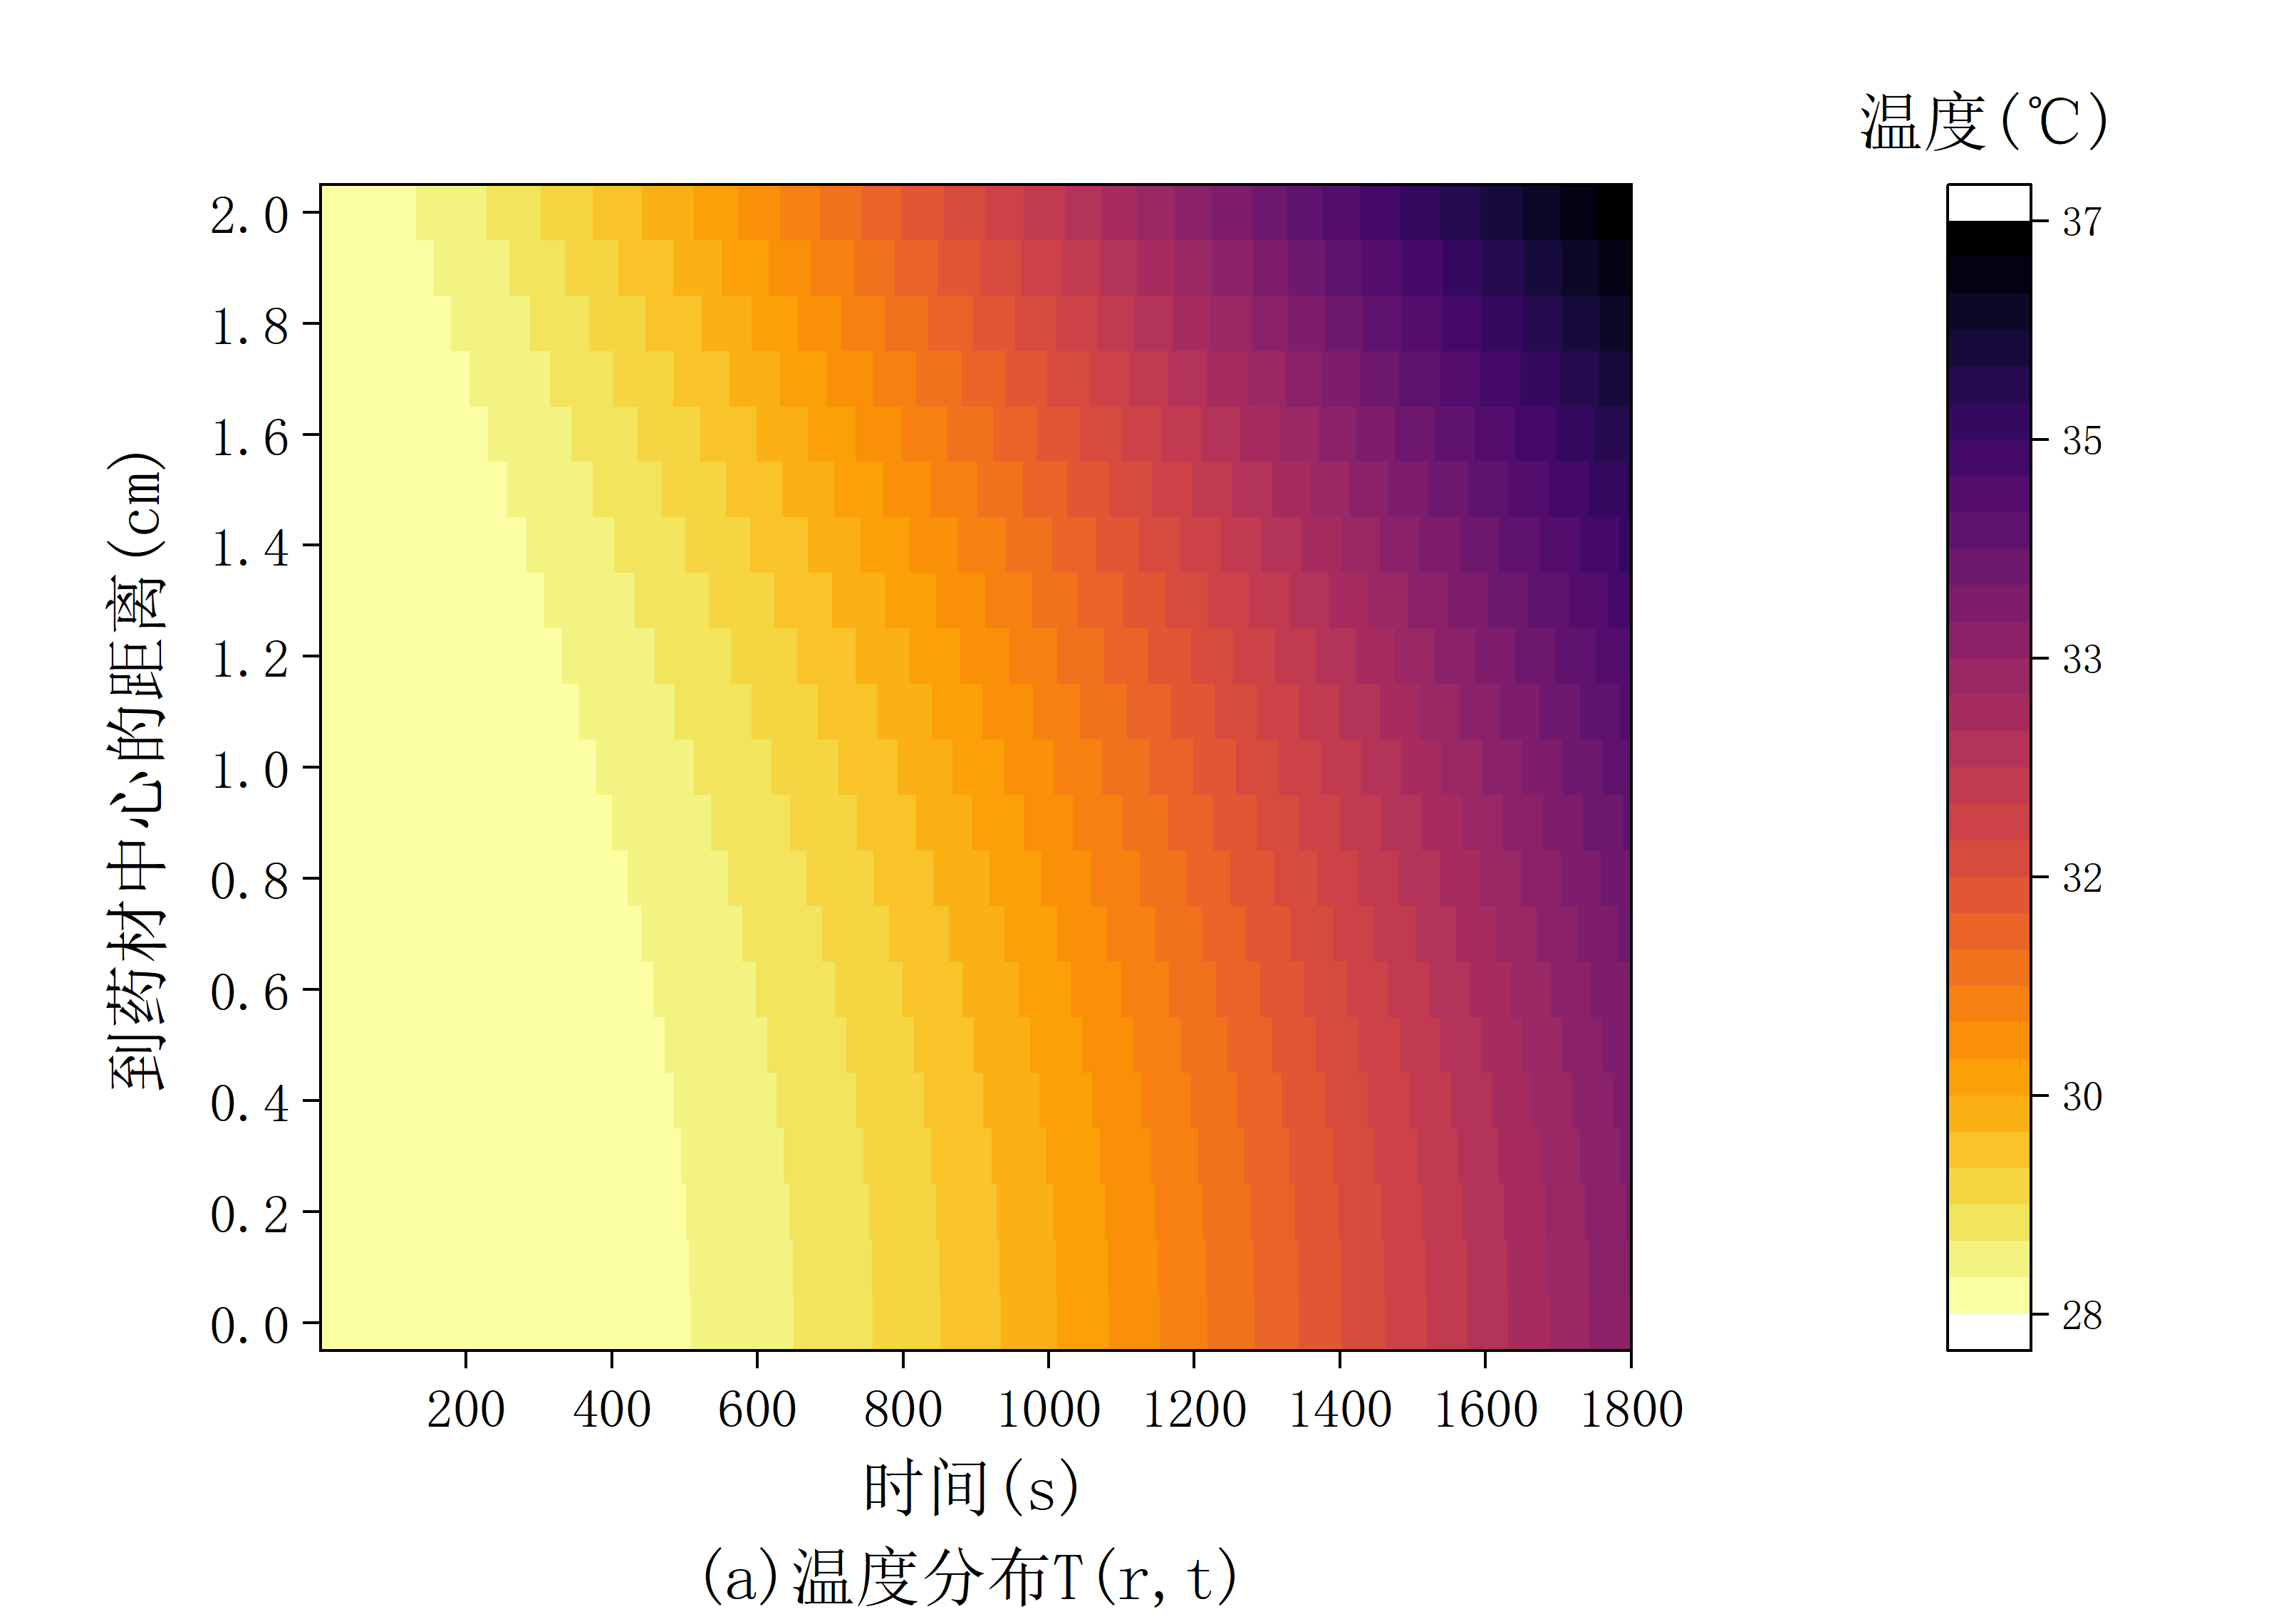
\includegraphics[trim={651.600bp 86.400bp 38.640bp 58.800bp},clip,
      height=0.329528822\unitlength]{图4(a).png}}}
  % ColorbarTitle
  \put(0.420549265,0.387170537){\makebox(0,0)[lb]{%
    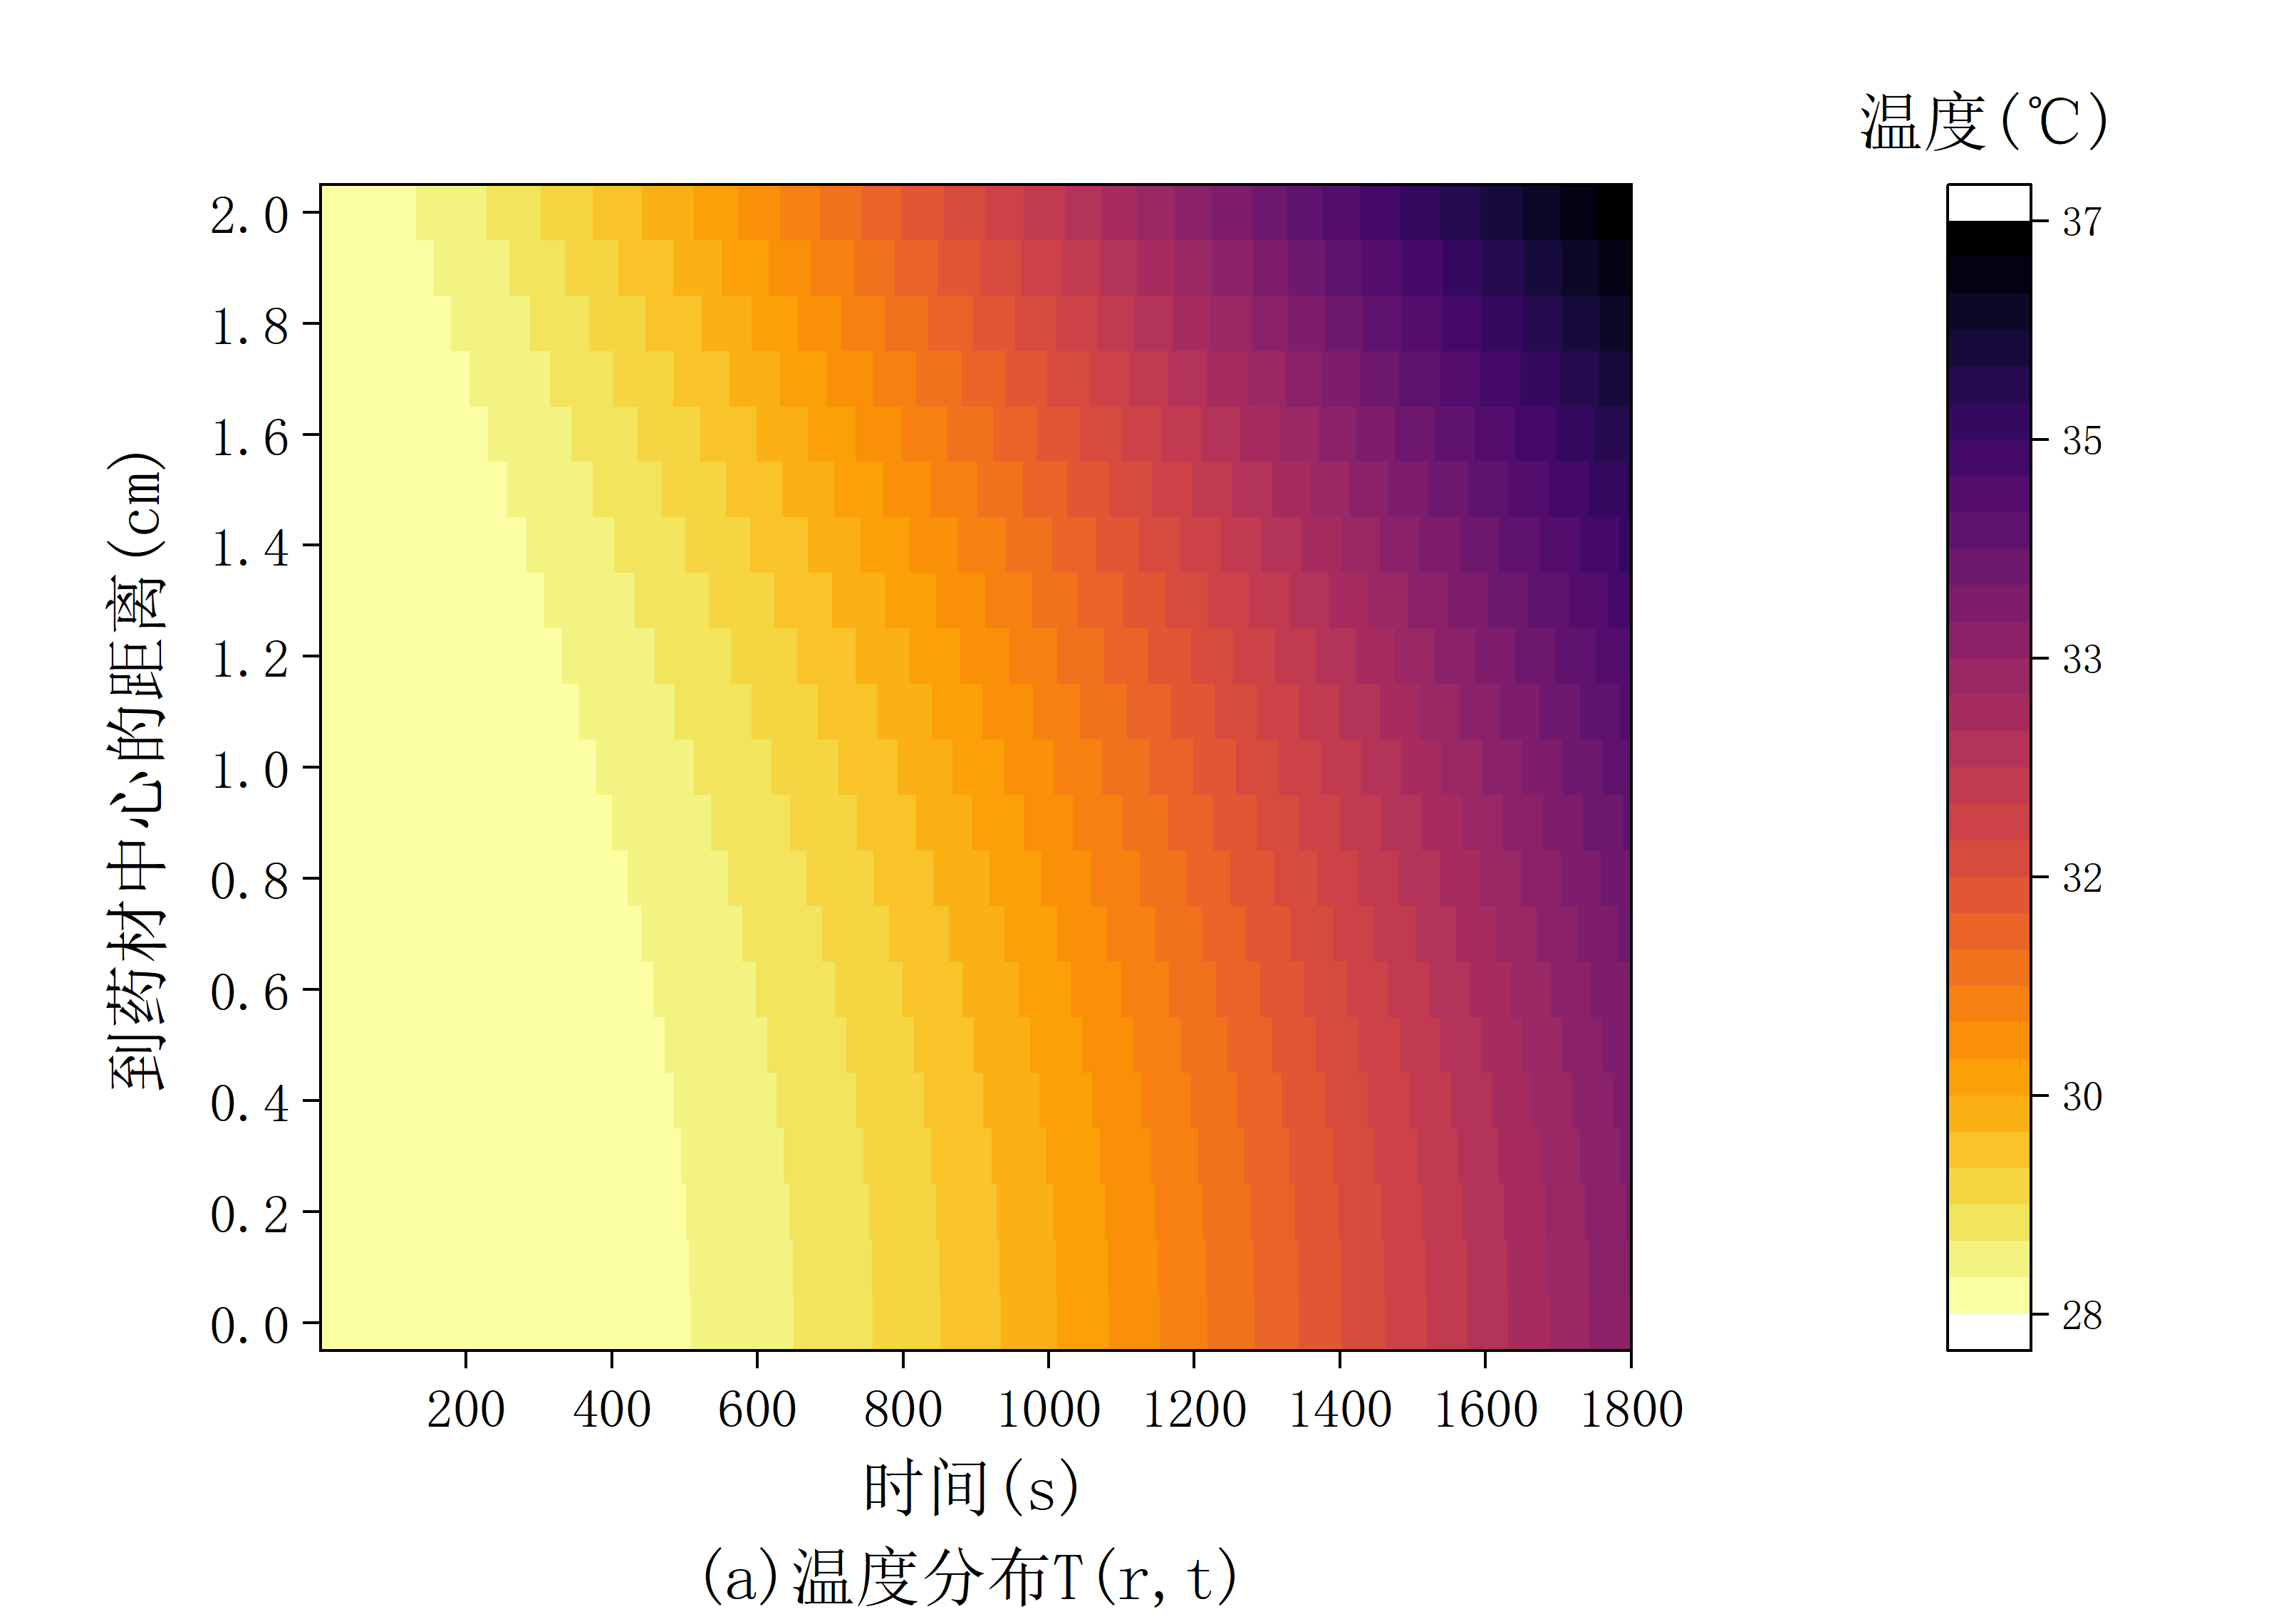
\includegraphics[trim={624.000bp 493.200bp 59.040bp 27.600bp},clip,
      height=0.021640699\unitlength]{图4(a).png}}}
  % B：仅指定高度，保持原PNG比例；向左利用空白间距。
  \put(0.513589096,0.013349051){\makebox(0,0)[lb]{%
    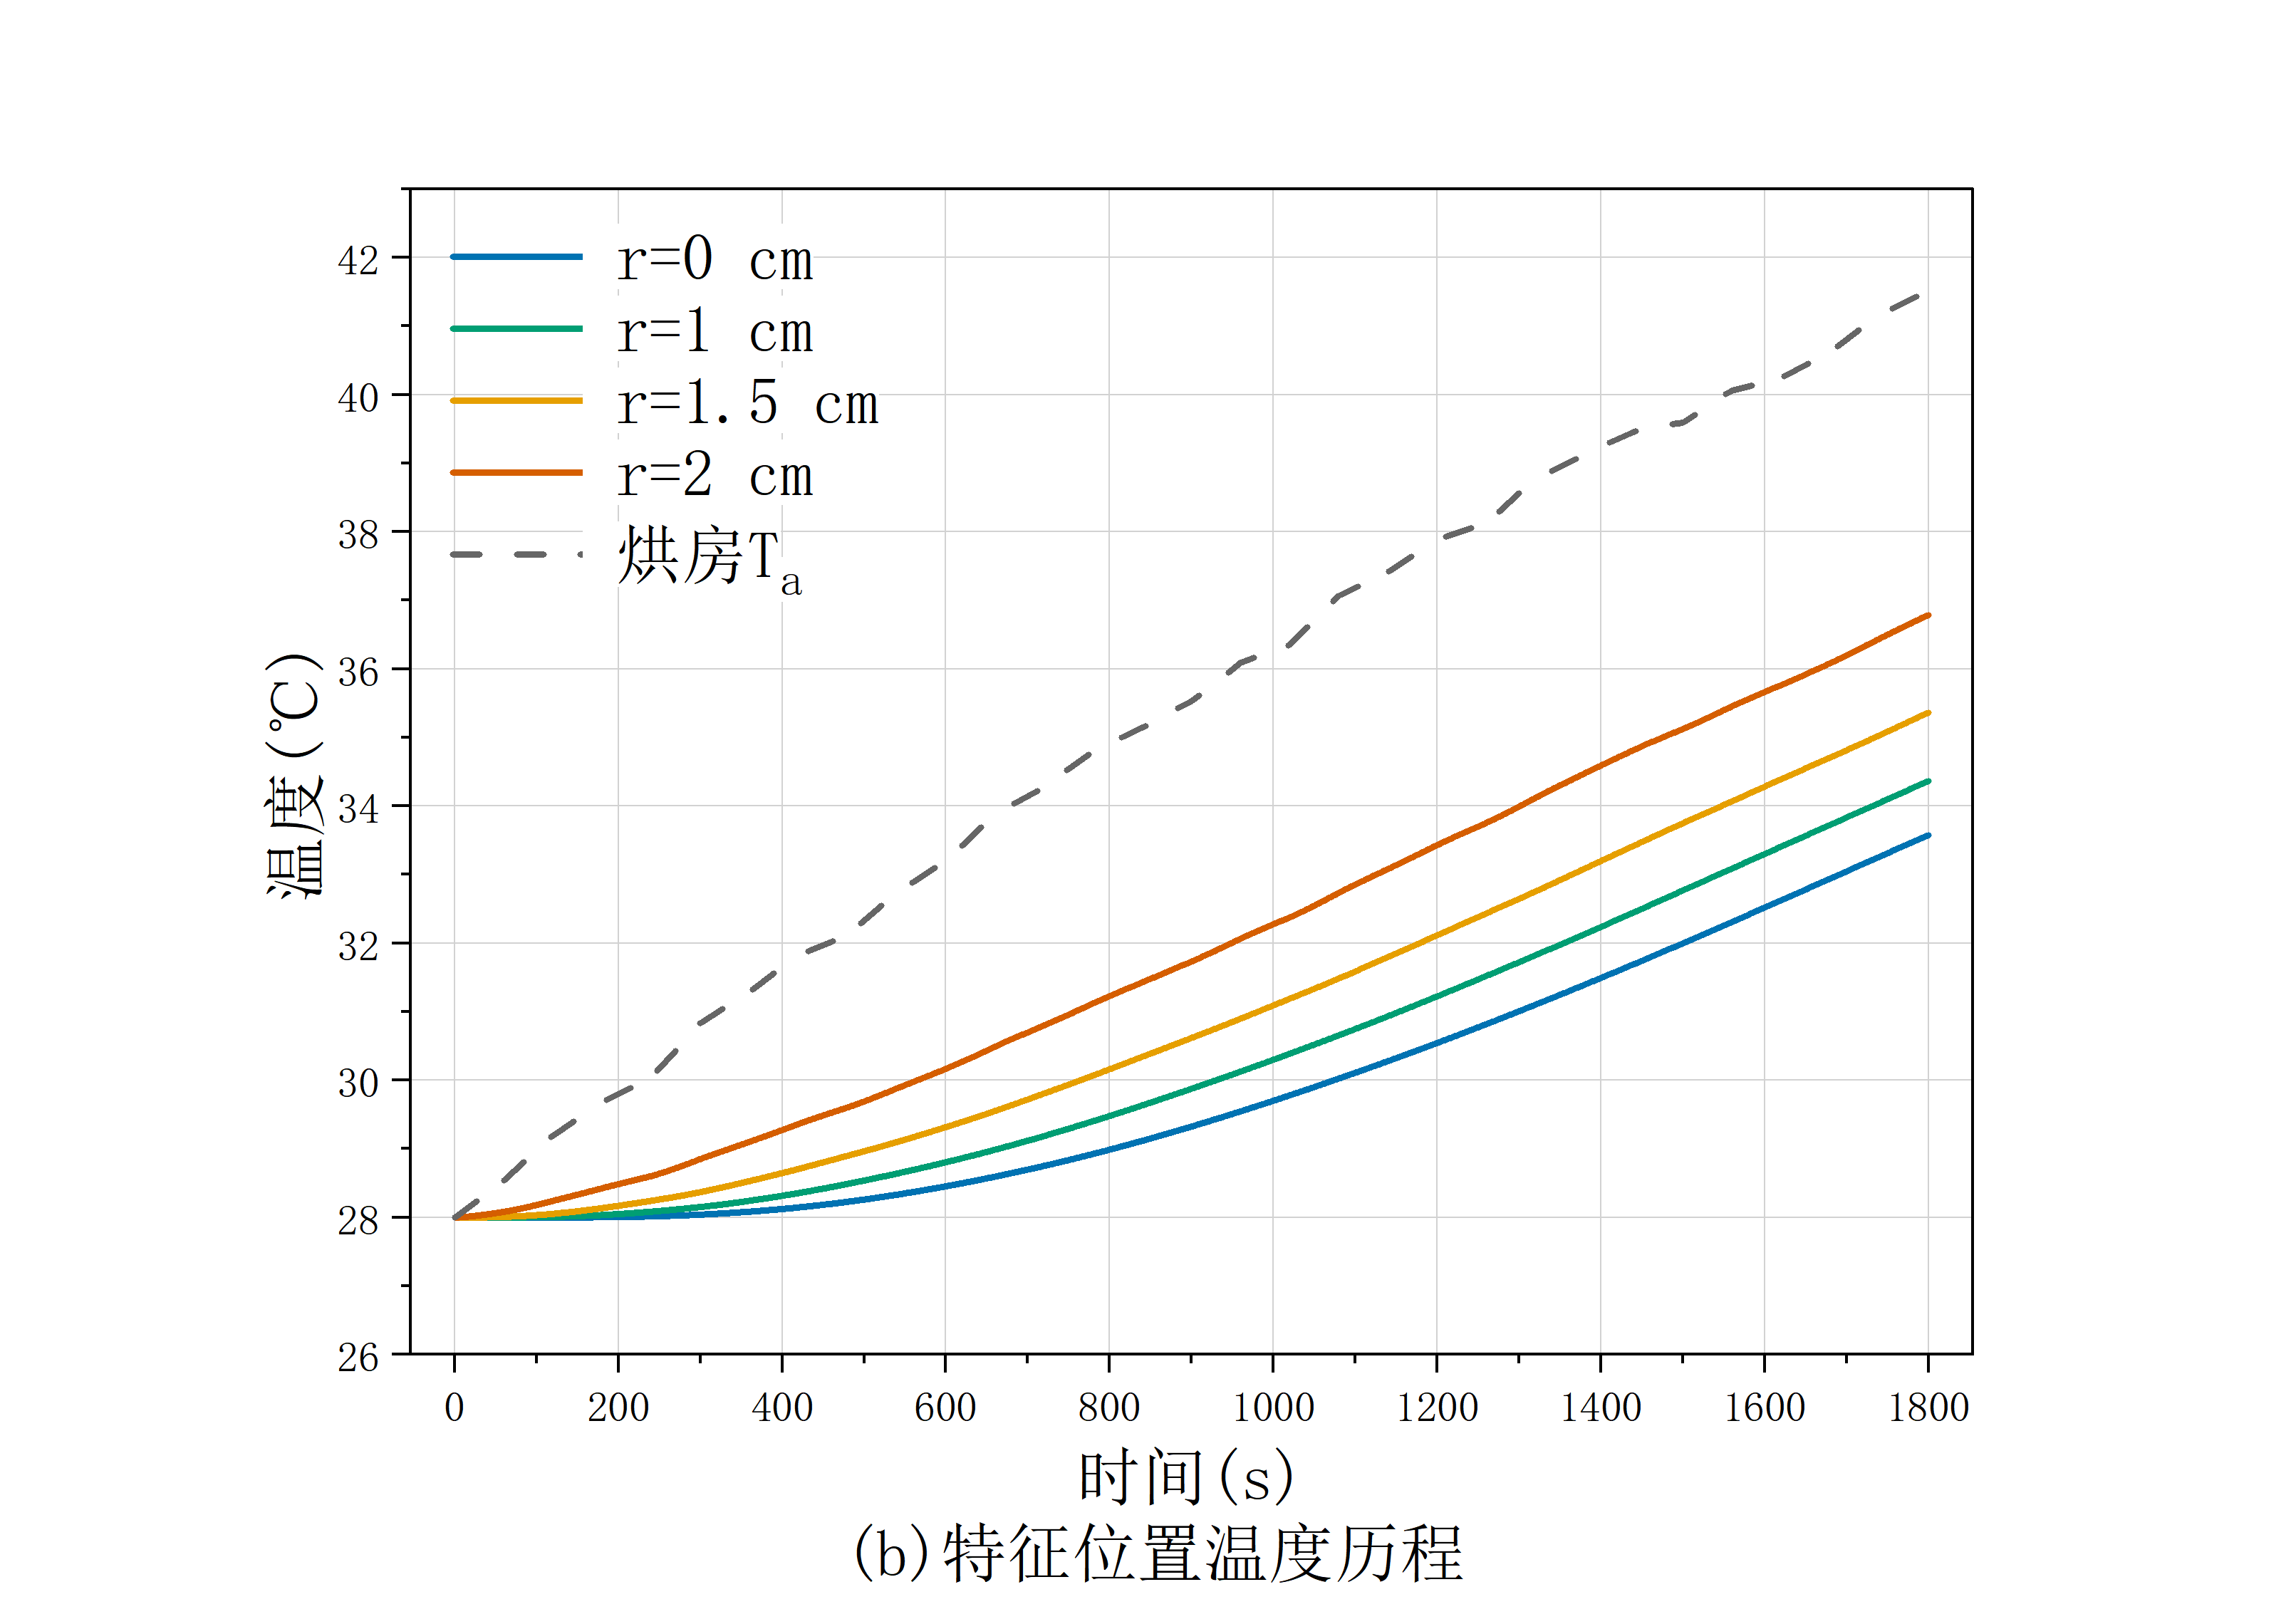
\includegraphics[trim={85.200bp 36.000bp 102.240bp 34.800bp},clip,
      height=0.390754948\unitlength]{图4(b).png}}}
\end{picture}
\caption{问题一温度场及特征位置温度历程}
\label{fig:p1-temperature}
\end{figure}

环境热量经表面对流输入，再由径向导热向内传递，有限的表面交换与内部导热能力形成上述温差。
因此，\textbf{30分钟时内部温度尚未均匀，药材与环境也未达到热平衡}。

\subsubsection{表层失水与热湿响应差异}

同期表面含水率由$2.55\cunit$降至$1.5102\cunit$，下降约$40.78\%$，
中心在表格显示精度下仍为$2.5500\cunit$。
图\ref{fig:p1-moisture}的径向剖面在内部平缓、近表面明显下降，
表明\textbf{前30分钟的显著失水主要集中于外层}。

\begin{figure}[!htbp]
\centering
% 保持原图4的0.98\textwidth宽度及264.62175/636.93875高宽比。
% 裁去白边并收紧(a)主图与色条的间距，完整保留两行色条标题。
% trim按源PNG的300 dpi换算；各部分仅指定高度，以保持原始比例。
\setlength{\unitlength}{0.98\textwidth}
\begin{picture}(1,0.415458708)
  % (a)水分场及坐标轴。
  \put(0.016642117,0.001726623){\makebox(0,0)[lb]{%
    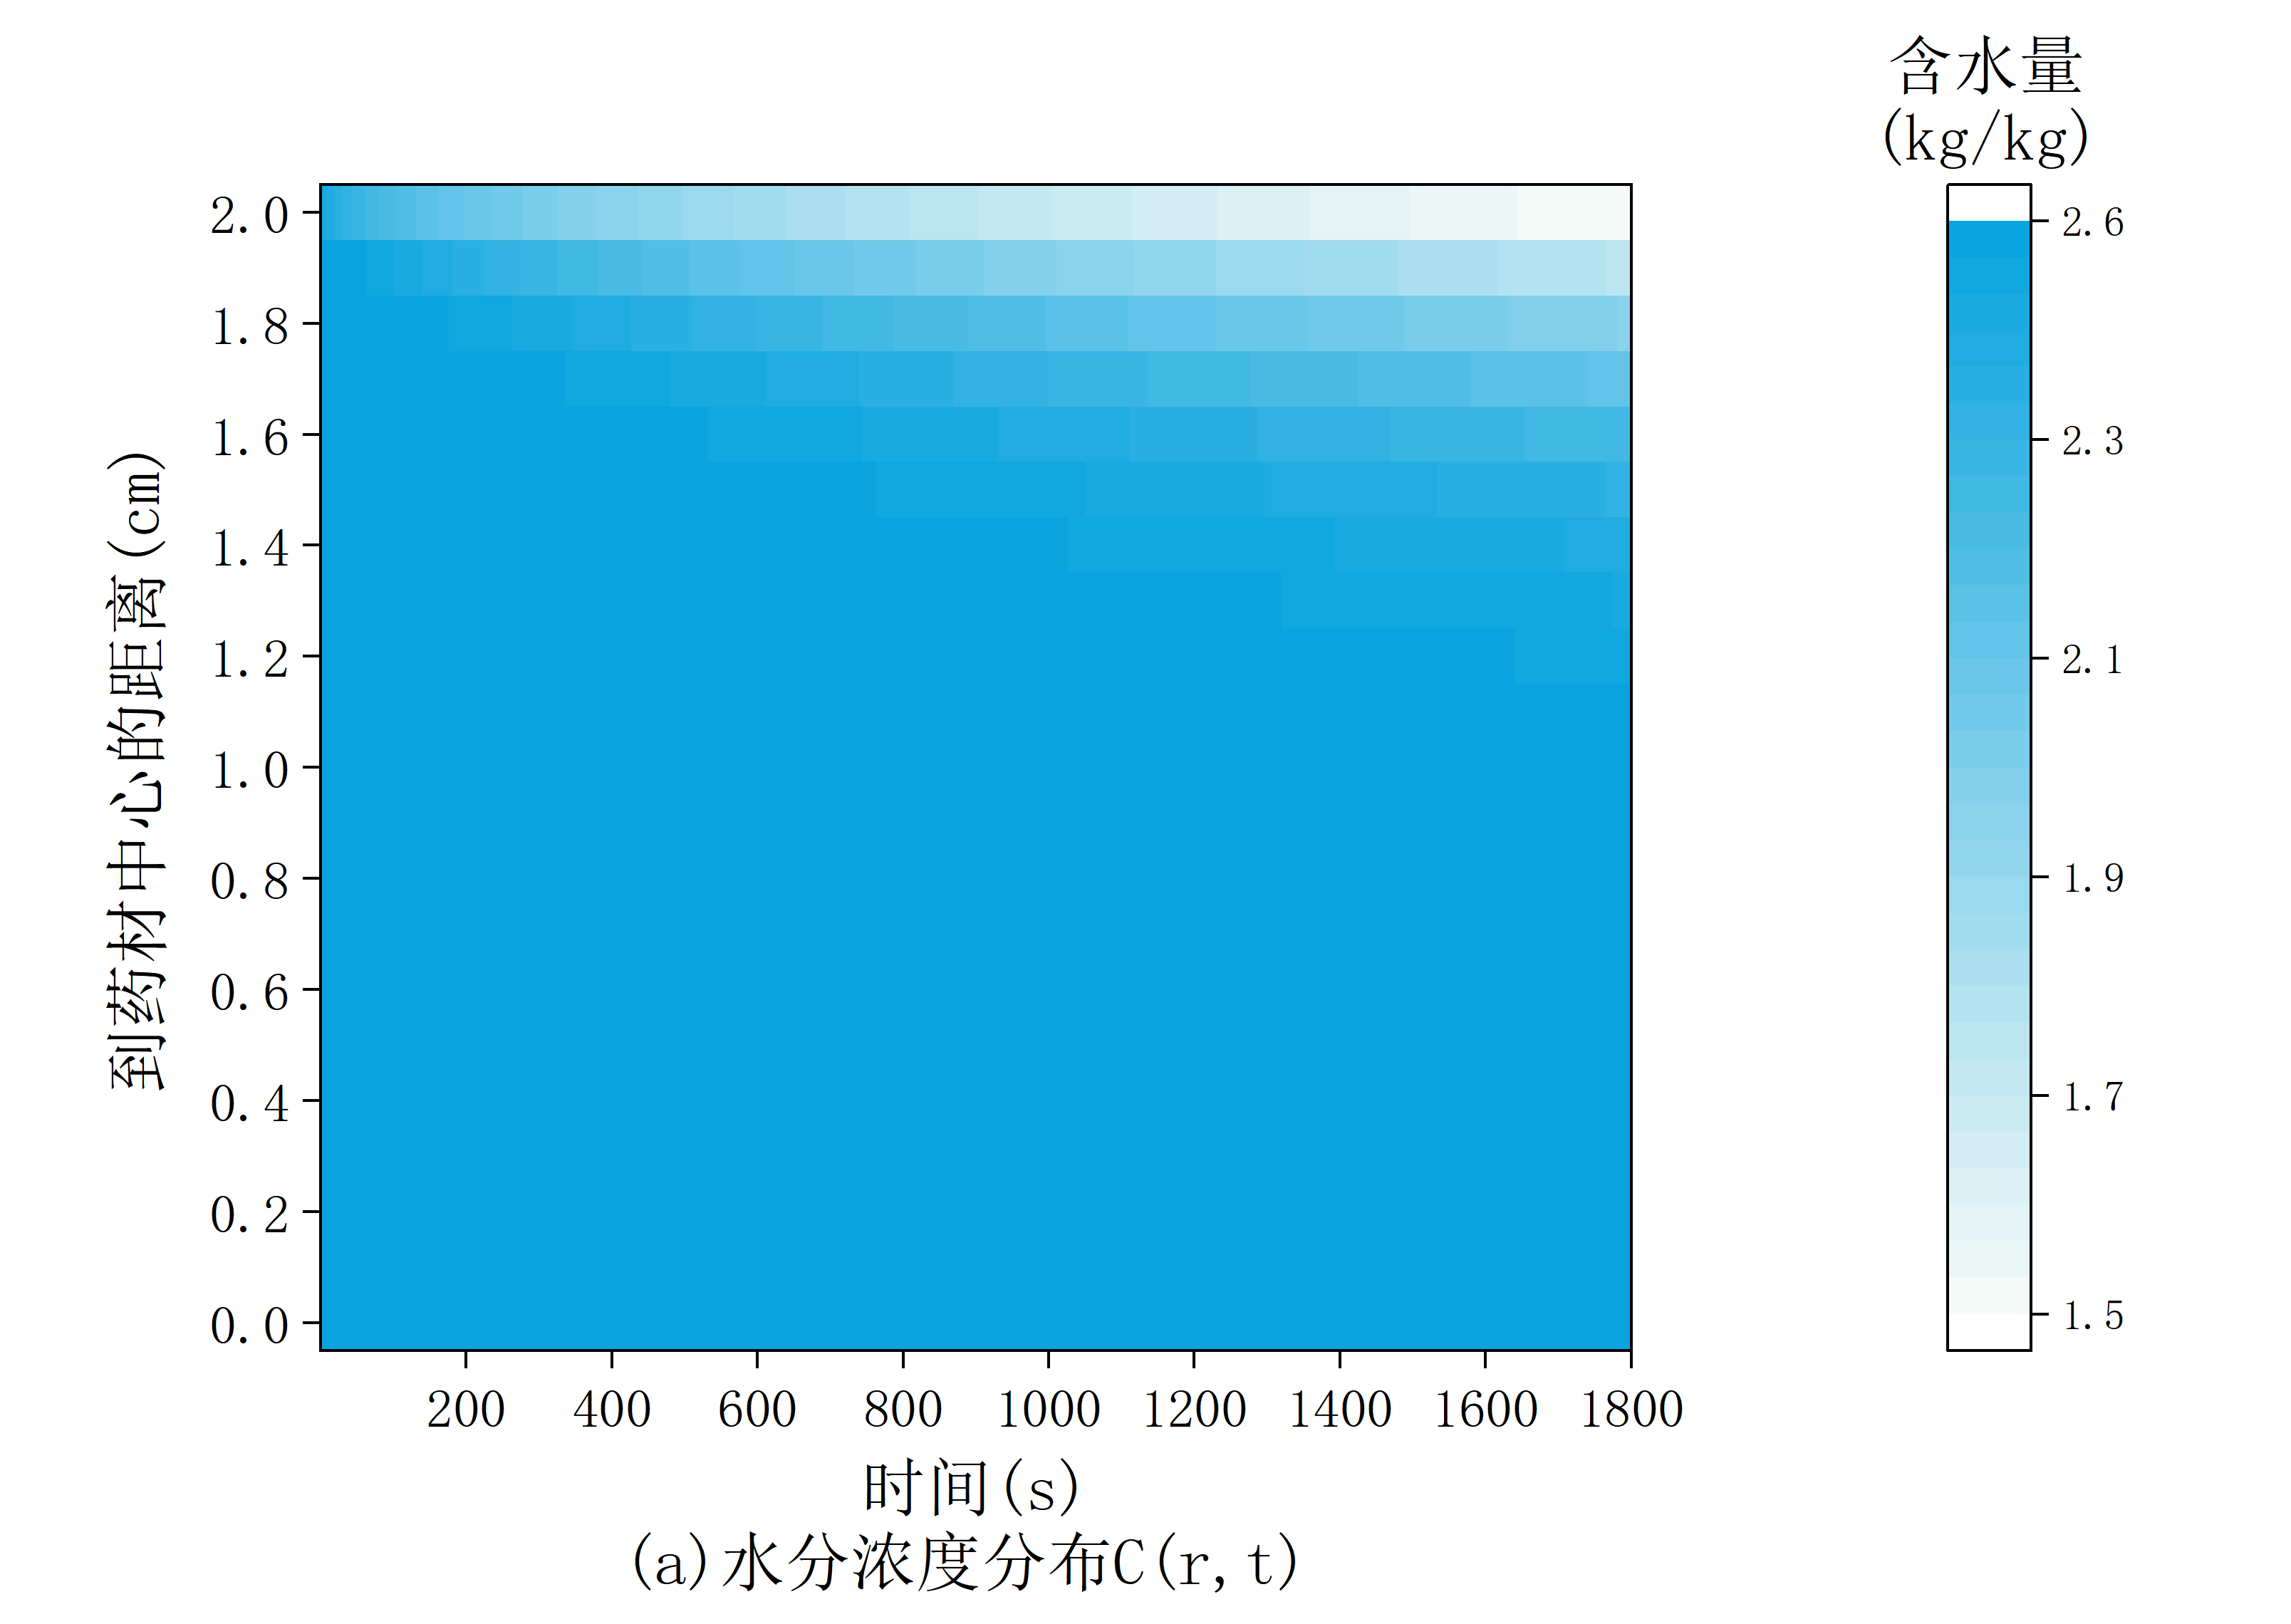
\includegraphics[trim={32.400bp 26.400bp 200.640bp 34.800bp},clip,
      height=0.392417307\unitlength]{图5(a).png}}}
  % (a)色条及其两行标题，与主图按相同比例缩放；分开裁剪避免白边覆盖主轴。
  \put(0.439628404,0.050173204){\makebox(0,0)[lb]{%
    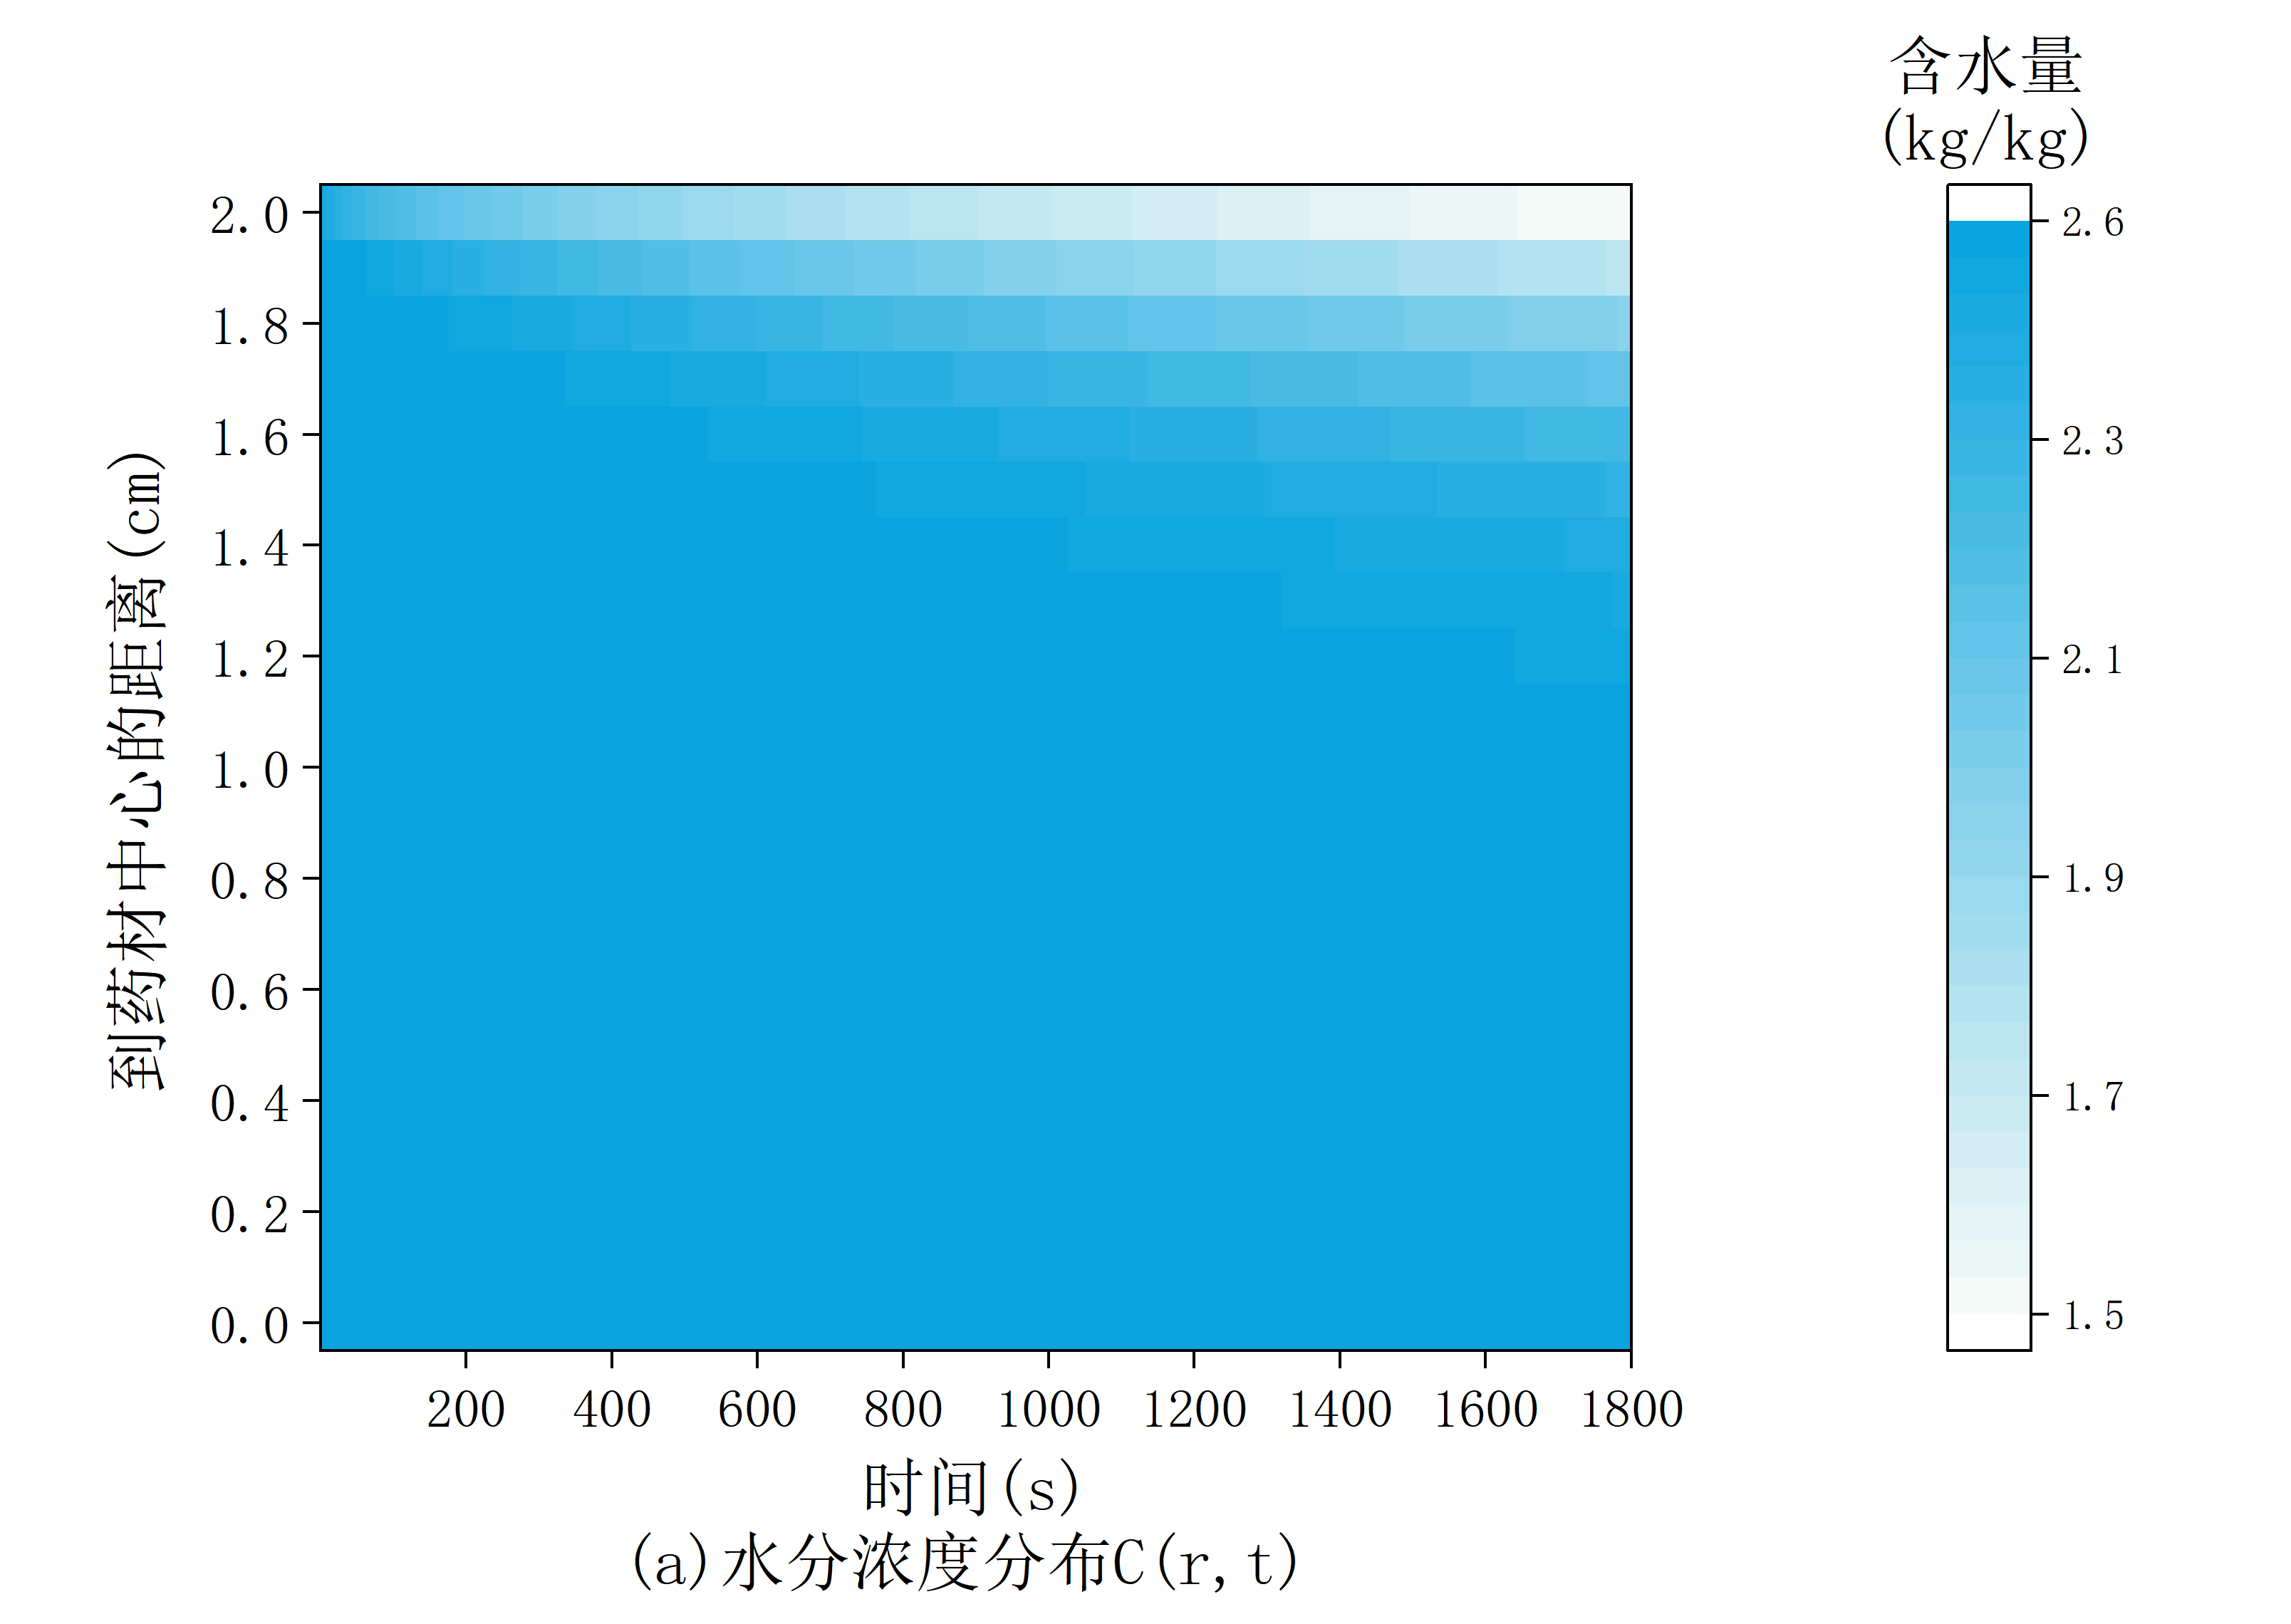
\includegraphics[trim={651.600bp 86.400bp 38.640bp 58.800bp},clip,
      height=0.324592094\unitlength]{图5(a).png}}}
  \put(0.424125498,0.374765298){\makebox(0,0)[lb]{%
    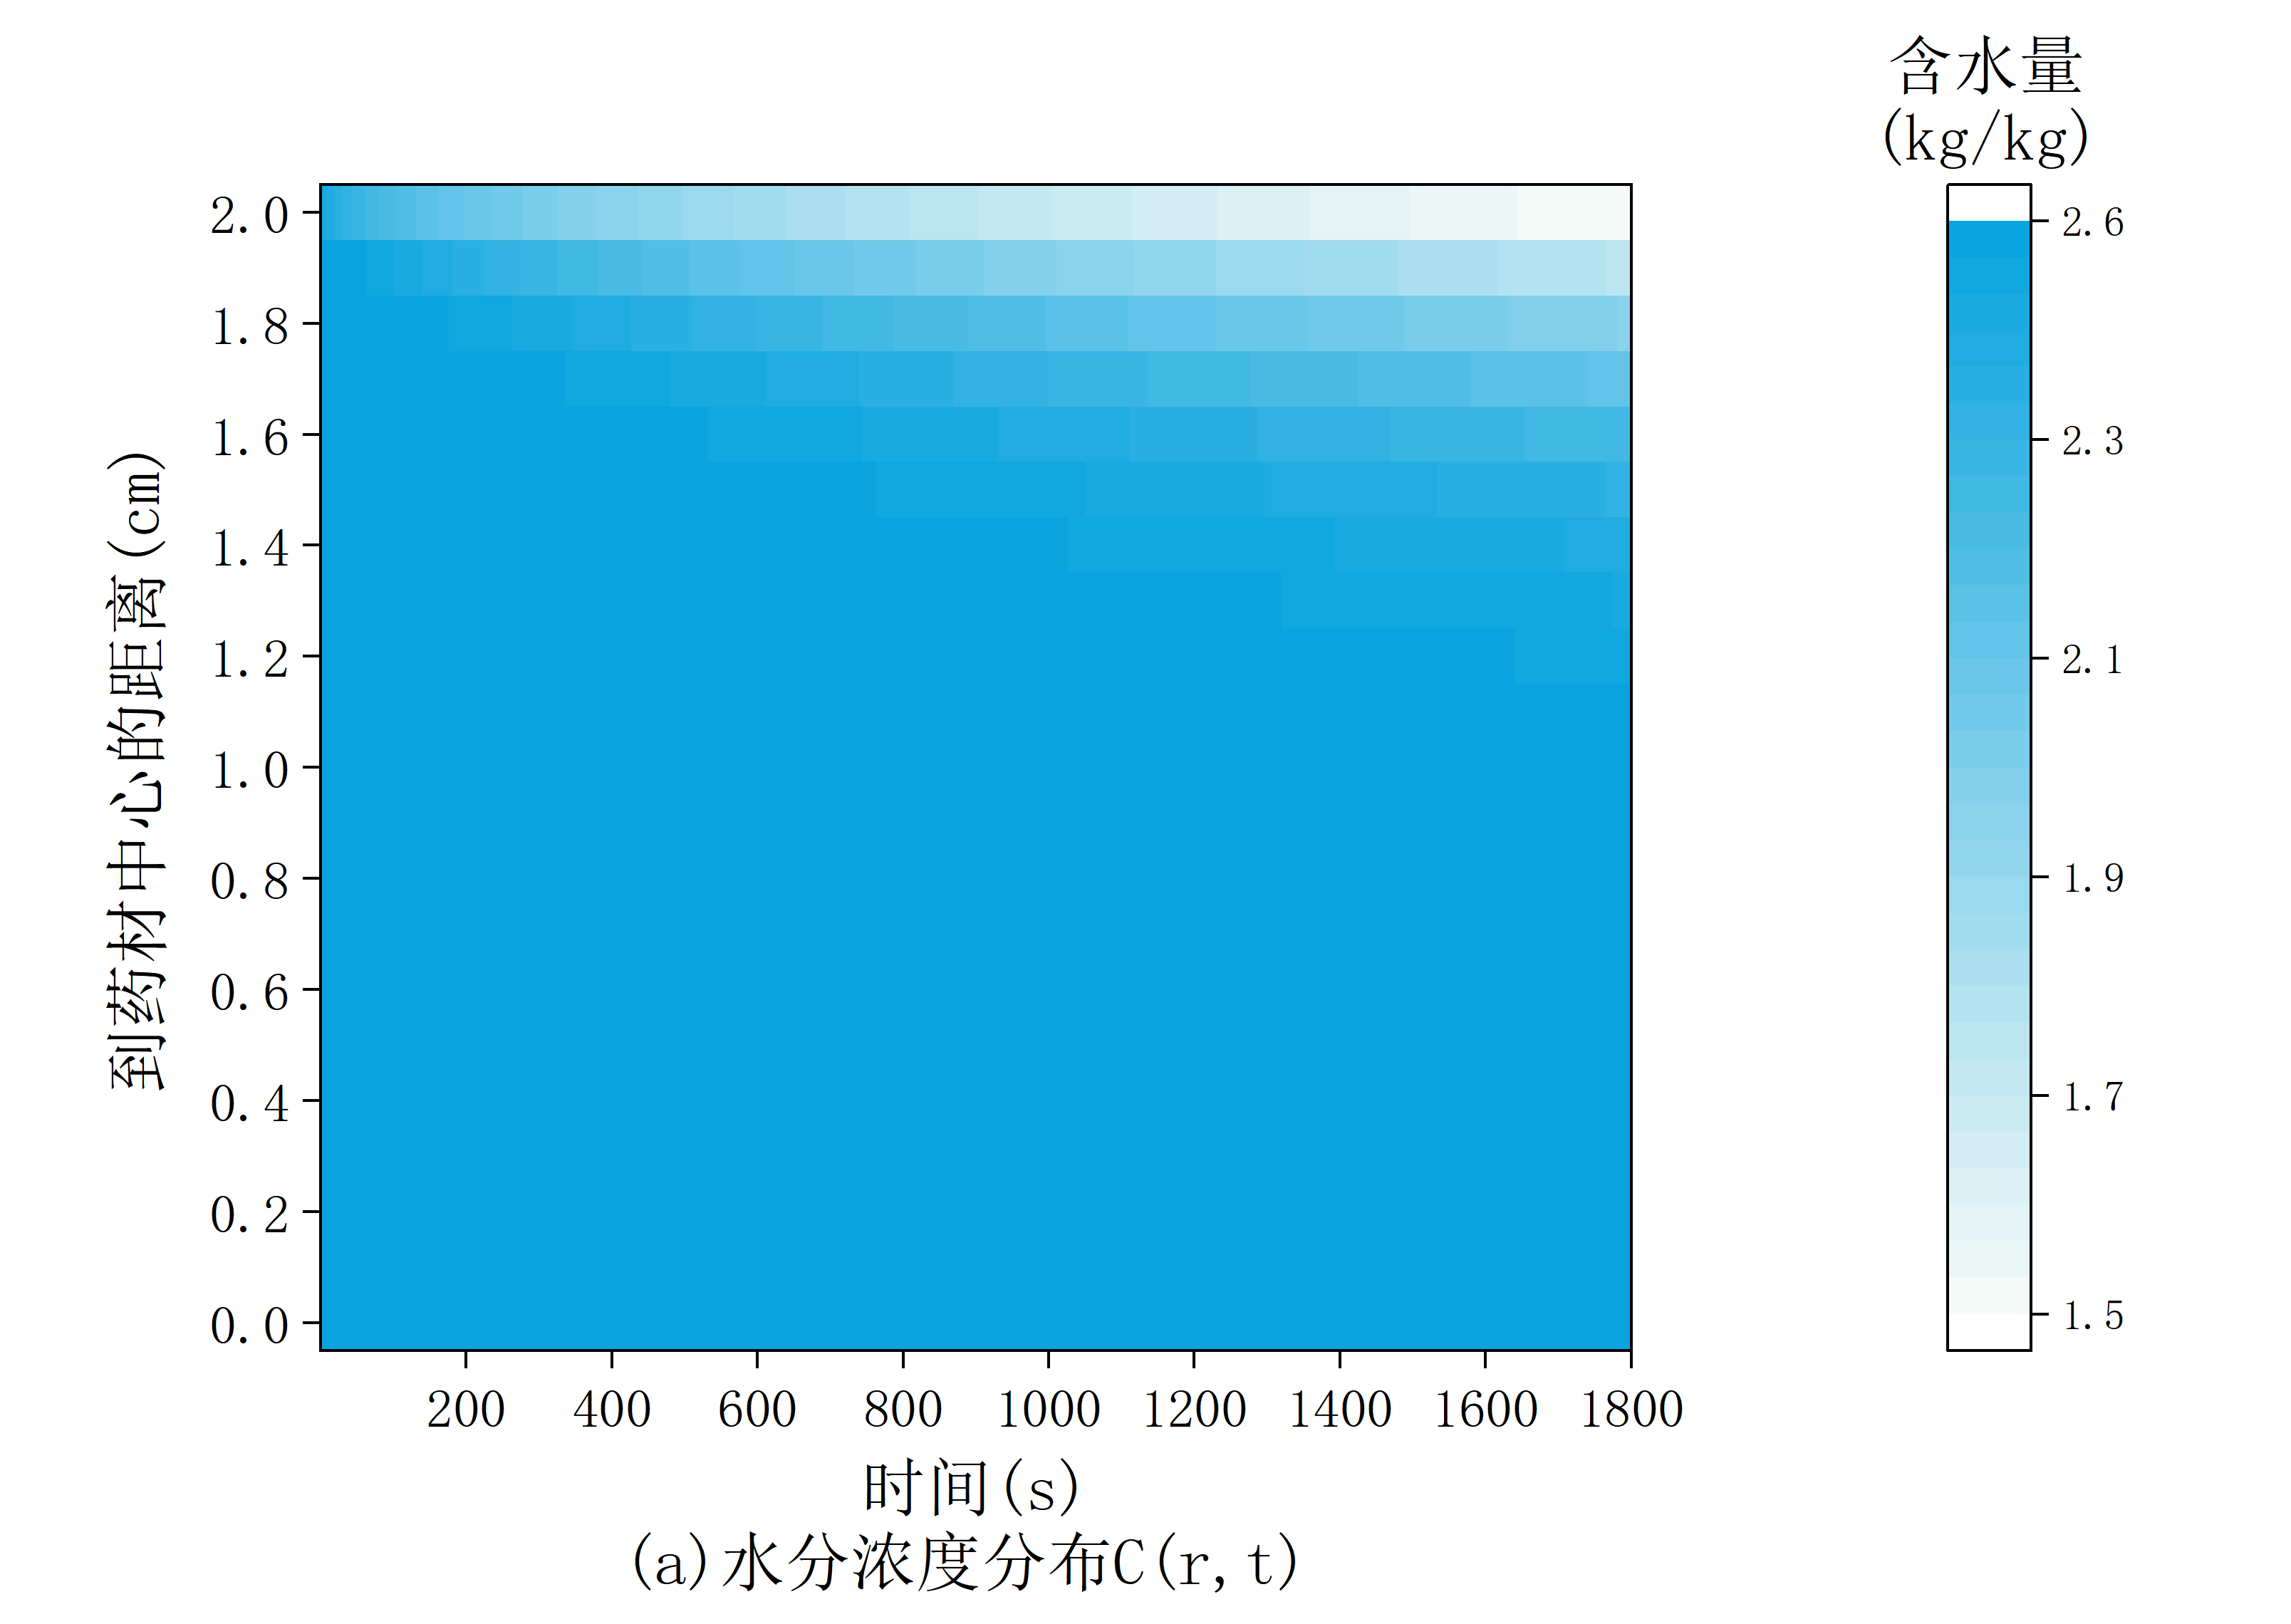
\includegraphics[trim={632.400bp 488.400bp 66.240bp 8.400bp},clip,
      height=0.040695128\unitlength]{图5(a).png}}}
  % (b)径向剖面，保持原比例，与(a)的轴框上下对齐。
  \put(0.514889610,0.010419823){\makebox(0,0)[lb]{%
    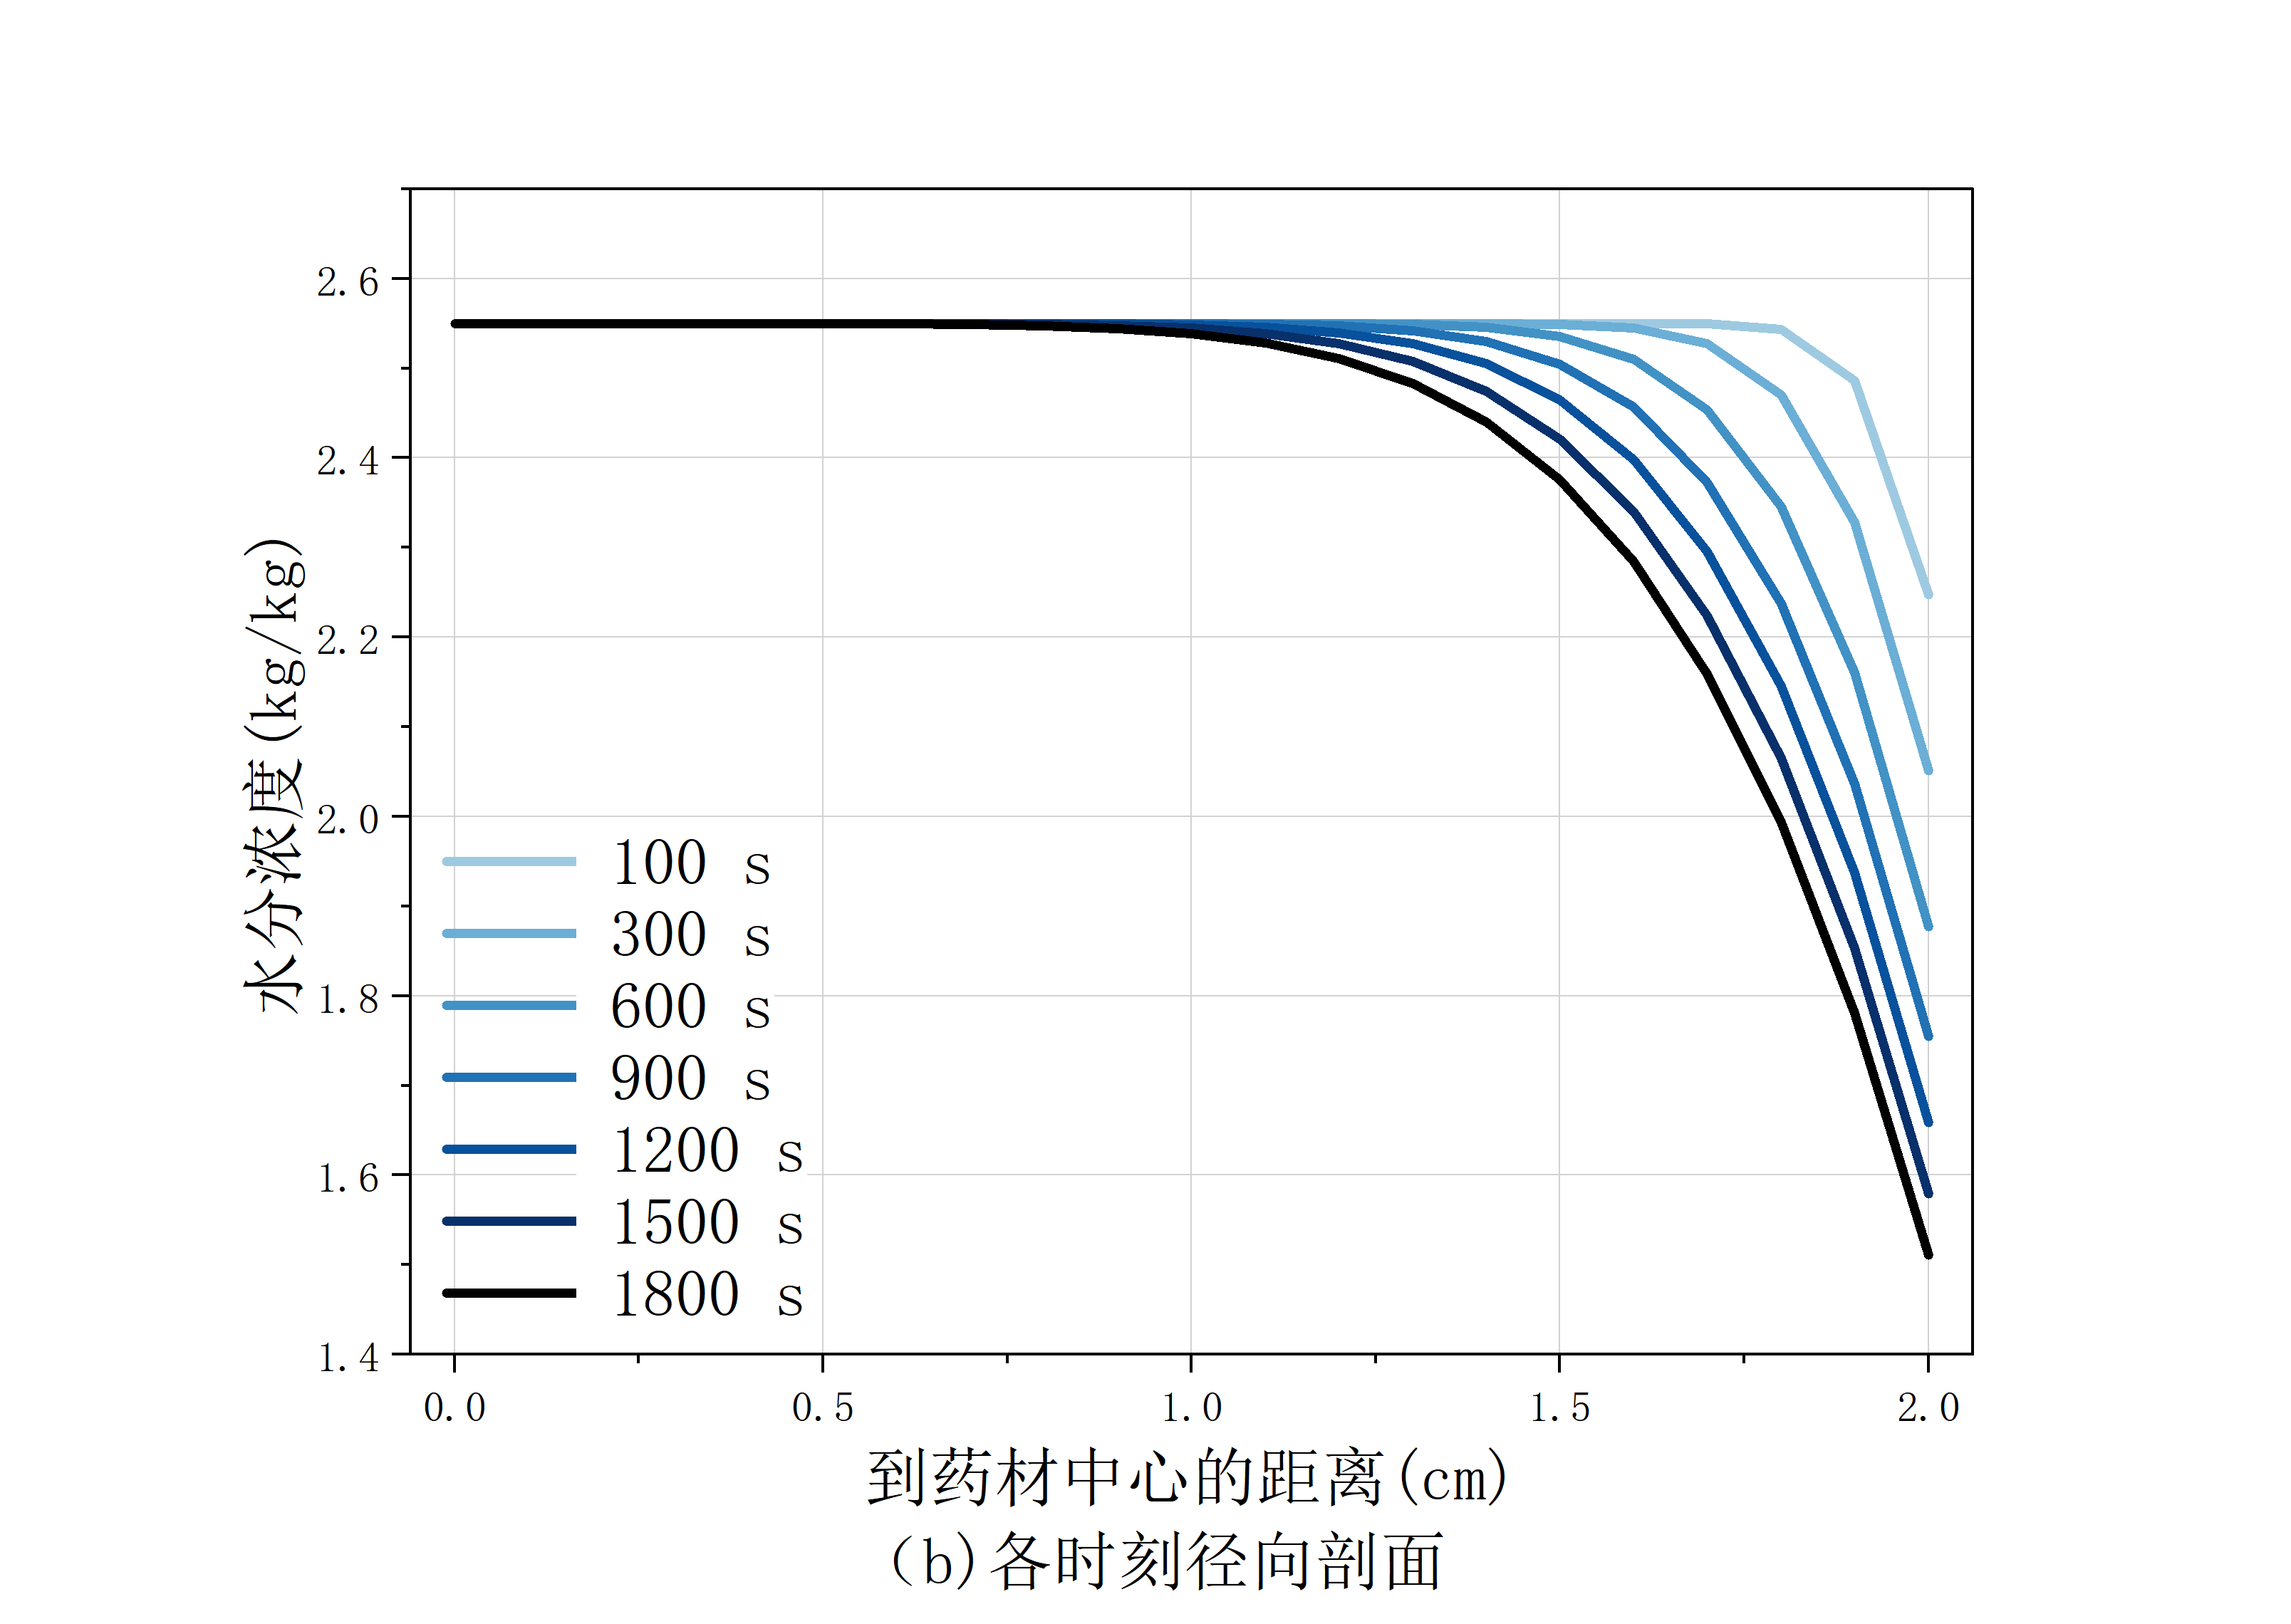
\includegraphics[trim={78.000bp 36.000bp 102.240bp 34.800bp},clip,
      height=0.384900980\unitlength]{图5(b).png}}}
\end{picture}
\caption{问题一水分场及不同时刻的径向含水率剖面}
\label{fig:p1-moisture}
\end{figure}

由式\eqref{eq:p1-biot}，热、质毕渥数分别为$1.3889$和$3.2404$，
两场均存在不可忽略的内部传递阻力，且水分内部扩散相对于表面交换受到的限制更突出。
外层失水使$D(C)$减小、传质毕渥数进一步增大，因此\textbf{表层先失水，内部水分补给滞后}。
毕渥数反映阻力比例，响应先后还取决于传递时间尺度：热扩散率
$\alpha=k/(\rho c_p)\approx1.69\times10^{-7}\ \mathrm{m^2/s}$约为$D(C_0)$的$34.2$倍，
同一径向尺度下热量向内传播更快；结合中心已经升温而含水率基本不变的结果，
可见\textbf{温度变化的影响先深入内部，内部失水响应相对滞后}。
